\qrchapter{https://forgottenpillar.com/rsc/sw-fp-chapter13}{Mungu wa Sabato v. Mungu wa Jumapili - J. B. Frisbie}

Kuna makala nyingine zilizoandikwa juu ya \emcap{Umbile la Mungu} na waanzilishi wetu na itakuwa kupita zaidi kujumuisha kila kitu hapa, lakini tungependa kuongeza ushuhuda mmoja zaidi kutoka kwa makala ya kaka J. B. Frisbie ambapo analinganisha Mungu wa Sabato na Mungu wa Jumapili. Yeye analinganisha ukweli juu ya \emcap{Umbile la Mungu} unaoonyeshwa katika hoja ya kwanza ya \emcap{Kanuni za Msingi} na fundisho la Utatu. Hebu tuangalie sehemu ya makala yake, “\textit{Sabato ya Siku ya Saba Haijakomeshwa}” kutoka kwa Review and Herald, Machi 7, 1854.

\begin{figure}[hp]
    \centering
    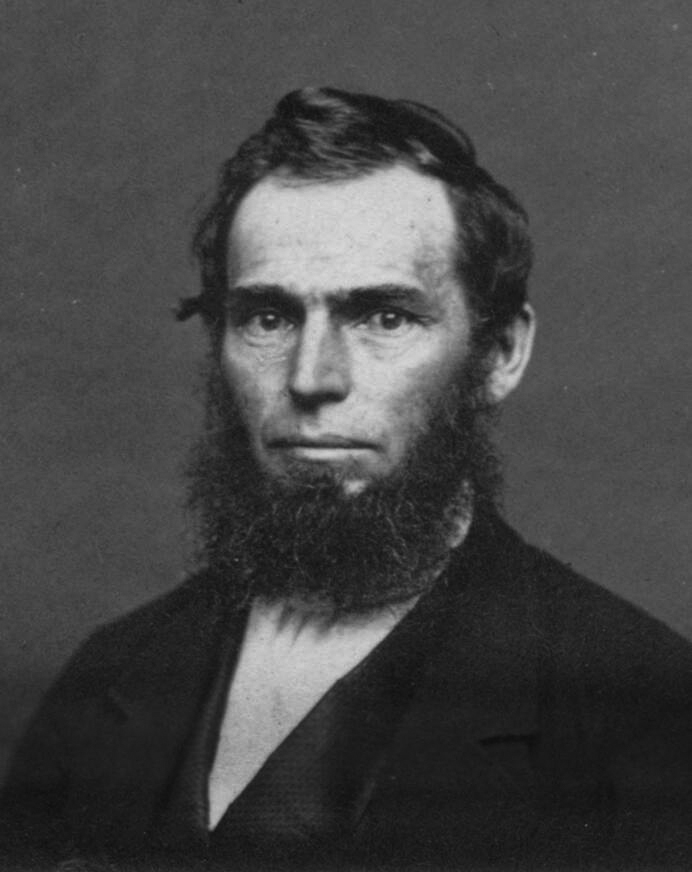
\includegraphics[width=1\linewidth]{images/j-b-frisbie.jpg}
    \caption*{John Byington Frisbie (1816-1882)}
    \label{fig:j-b-frisbie}
\end{figure}

\section*{Mungu wa Sabato}

\others{Baada ya kumjua na kumkumbuka Mungu, kwa kutunza Sabato yake takatifu, \textbf{basi Biblia itafundisha kuhusu ubinafsi wake na makazi yake}. \textbf{Mwanadamu yuko katika sura na mfano wa Mungu}. Mwanzo 1:26. ‘Mungu akasema, (akisema na mwanawe) na tumfanye mwanadamu kwa mfano wetu, baada ya namna yetu’. Sura ya 2:7. ‘Bwana Mungu akamuumba mwanadamu kwa mavumbi ya ardhi, akampulizia pumzi puani mwake, pumzi ya uhai; mtu akawa nafsi hai’. Mwanzo 9:6; 1 Wakorintho 11:7; Yakobo 3:9. \textbf{Kile kilichofanywa kwa \underline{sura na mfano wa Mungu} kilifanywa kwa mavumbi ya ardhi kiliitwa mwanadamu}.}

\othersnogap{Hii inajulikana kuwa maana ya kweli kutoka kwa ushuhuda mwingine ambao umeweza kutolewa kutoka kwa Biblia. \textbf{Yesu alikuwa katika umbo la mwanadamu na sura ya wazi ya nafsi wa Baba yake}.}

\othersnogap{Wafilipi 2:6-8. \textbf{Kristo Yesu}: ‘Ambaye alikuwa yu katika \textbf{fomu ya Mungu}, naye hakuona kuwa ni unyang'anyi kuwa \textbf{sawa na Mungu}. Bali alijifanya kuwa hana sifa, akatwaa \textbf{fomu ya mtumishi}, \textbf{akafanywa kwa fomu ya wanadamu}’. 2 Wakorintho 4:4. \textbf{‘Na kufanywa mtindo kama mwanadamu’}, n.k. Wakolosai 1:15. ‘\textbf{Yeye aliye mfano wa Mungu asiyeonekana}’.}

\othersnogap{Waebrania 1:3. \textbf{Mwana; ‘Ambaye kwa kuwa ni mng'ao wa utukufu wake, na chapa iliyo dhahiri ya nafsi yake’}. Kwa namna hii Yesu angeweza kumwambia Filipo kwa kweli, ‘Yeye aliyeniona amemwona Baba.’ Yoh. 14:9. Wengine wanaonekana kudhani kuwa \textbf{inapingana na ubinafsi wa Mungu, \underline{kwa sababu yeye ni Roho, na husema kwamba yeye hana mwili, au viungo}}. Yohana 4:24. ‘\textbf{Mungu ni Roho}’. Waebrania 1:7. ‘\textbf{Nani afanyaye malaika zake kuwa roho}’. \textbf{Nani atajifanya kusema kwamba malaika hawana miili au sehemu kwa sababu wao ni roho}. \textbf{\underline{Hata hivyo Mungu ni huluki ya kiroho mwenye mwili na viungo kama tunavyoweza kujifunza kwa kuwa ana makao na kwa sababu anayo na anaweza kuonekana}}. Kutoka 33:23. ‘Nami nitauondoa mkono wangu, nawe \textbf{utaona sehemu zangu za nyuma}, lakini \textbf{uso wangu hautaonekana}’. Mathayo 5:8. ‘Wamebarikiwa walio safi moyoni, maana hao \textbf{watamwona Mungu}’. Waebrania 12:14. ‘Fuata amani na watu wote, na utakatifu, pasipo hayo\textbf{mtu atakayemwona Bwana} asipokuwa nao’. Mathayo 18:10. ‘mle mbinguni malaika wao siku zote \textbf{huutazama uso wa Baba yangu aliye mbinguni}’. Mathayo 6:9. ‘Basi ninyi salini hivi, \textbf{Baba yetu uliye mbinguni}’, nk. Yohana 6:38. ‘Kwa mimi \textbf{nilishuka kutoka mbinguni} si kufanya mapenzi yangu mwenyewe, bali mapenzi yake aliyenituma’. Sura 16:28. ‘\textbf{Nilitoka kwa Baba, nami nimekuja ulimwenguni}: tena \textbf{nawaacha duniani, naenda kwa Baba}’.}

\othersnogap{\textbf{Je, Mungu hasemi kwamba anajaza ukubwa wa anga? \underline{Tunajibu, La}}. Zaburi 139:7, 8. ‘Nenda wapi niiache \textbf{Roho yako}? au nitakimbilia wapi nijiepushe \textbf{na uwepo wako}? Nikipanda juu mbinguni, wewe uko’, n.k. \textbf{\underline{Mungu kwa Roho wake aweza kujaza mbingu na nchi}}, nk. \textbf{Watu humchanganyisha Mungu na Roho wake, ambayo huleta machafuko}. Zaburi 11:4. ‘\textbf{Bwana yu ndani ya hekalu lake takatifu, kiti cha enzi cha Bwana ki mbinguni}: macho yake yanaona’, nk. Habakuki 2:20; Zaburi 102:19. ‘Maana ametazama chini \textbf{kutoka mahali palipoinuka pa patakatifu pake}; \textbf{\underline{kutoka mbinguni} Bwana alitazama dunia}’. 1 Petro 3:12. ‘Kwa maana macho ya Bwana huwaelekea wenye haki, na masikio yake husikiliza maombi yao’, n.k. Zaburi 80:1. ‘Sikia, Ee Mchungaji wa Israeli, wewe unayemwongoza Yusufu kama kundi; wewe \textbf{ukaaye kati ya makerubi}, angaza’. Zaburi 99:1; Isaya 37:16.}

\othersnogap{Yohana 14:2. ‘Nyumbani mwa Baba yangu mna makao mengi. naenda kuwaandalia mahali’. Ufunuo 21:2-5; Waebrania 11:6. ‘Kwa maana mtu amwendeaye Mungu lazima aamini kwamba yeye yuko’, nk. \textbf{Ushuhuda huu tunauona kuwa umuhimu sana wakati huu, kujua kwamba kuna Mungu. Sisi hatuna shaka kwamba ikiwa macho yetu yangeweza kufunguliwa katika maono, au kuona kama malaika wanavyoona, sisi kumwona Mungu mbinguni ameketi katika kiti chake cha enzi, naye yuko kwa vitu vyote vilivyoko; ingawaje vi mbali naye katika uumbaji wake}.}[\href{https://documents.adventistarchives.org/Periodicals/RH/RH18540307-V05-07.pdf}{Adventist Review and Sabbath Herald, March 7, 1854}, J. B. Frisbie, “The Seventh-Day Sabbath Not Abolished”, p. 50]

Hapa tunaona hoja na fikra sawa, kwamba Mungu ni huluki wa kiroho wa kibinafsi. Mungu huyu ni Mungu wa Sabato. Ndugu Frisbie anamlinganisha Mungu huyu na Mungu wa Jumapili, ambaye ni Mungu wa utatu.

\section*{Mungu wa Jumapili}

\others{Tutafanya dondoo chache, ili msomaji apate \textbf{kuona tofauti kubwa kati ya \underline{Mungu wa Biblia} anayedhihirishwa nuruni kwa kushika Sabato, na mungu aliye gizani kupitia utunzaji wa Jumapili}. Katekisimu ya Kikatoliki Iliyofupishwa na Rt. Mchungaji John Dubois, Askofu wa New York. Ukurasa wa 5. ‘\textbf{Maswali. Mungu yuko wapi? Jibu. Mungu yuko kila mahali}. Swali. Je! Mungu anaona na kujua vitu vyote? A. Ndiyo, anajua na kuona vitu vyote. \textbf{Swali. Ana Mungu mwili wowote? Jibu. \underline{Hapana; Mungu hana mwili, ni Roho safi}}. \textbf{Swali. Je, kuna Miungu zaidi ya mmoja? Jibu. Hapana; kuna Mungu mmoja tu. Swali. Je, kuna nafsi zaidi ya moja katika Mungu? Jibu. \underline{Ndiyo; katika Mungu kuna nafsi tatu}. Swali. Ni zipi? Jibu. Mungu Baba, Mungu Mwana na Mungu Roho Mtakatifu. Swali. Je, hakuna Miungu watatu? Jibu. Hapana; Baba, Mwana na Roho Mtakatifu, wote ni Mungu mmoja tu}’.}

\othersnogap{Kifungu cha kwanza cha Dini ya Methodisti, uk. 8. \textbf{‘Kuna Mungu mmoja tu aliye hai na wa kweli}, milele, \textbf{bila mwili au sehemu}, mwenye nguvu isiyo na mwisho, hekima na wema: mtengenezaji na mhifadhi wa vitu vyote, vinavyoonekana na visivyoonekana. \textbf{Na katika umoja wa familia ya Uungu hii, wako nafsi watatu wa dutu moja, nguvu na umilele; Baba, Mwana, na Roho Mtakatifu}’.}

\othersnogap{Katika makala hii kama vile fundisho la Kikatoliki, \textbf{tunafundishwa kwamba kuna nafsi tatu za dutu moja,} nguvu na umilele katika yote \textbf{Mungu mmoja aliye hai na wa kweli}, milele \textbf{bila mwili au sehemu}. Lakini katika haya yote hatuambiwi \textbf{kilichotokea kwa mwili wa Yesu aliyekuwa na mwili alipopaa, aliyekwenda kwa Mungu ambaye ‘yuko kila mahali’ au hayuko popote}. Dokolojia.}

\othersnogap{‘\textbf{Kwa Mungu Baba, Mungu Mwana,}} \\
\others{\textbf{Mungu Roho, watatu katika mmoja}.’} \\
\others{Tena} \\
\others{‘Hupea joto jua, huburudisha kwenye upepo,} \\
\others{Anang'aa katika nyota, na maua katika miti.} \\
\others{\textbf{Anaishi katika maisha yote, anaenea kwa kiwango chochote},} \\
\others{Huenea bila kugawanywa na hufanya kazi bila matumizi.’ - Papa.}

\othersnogap{Mawazo haya yanapatana vyema na wale wanafalsafa wapagani. Mmoja anasema, ‘Maji hayo yalikuwa kanuni ya vitu vyote, na kwamba Mungu ndiye akili, ambaye kupitia kwake vitu vyote vinatengenezwa na maji.’ Mwingine, ‘Hewa hiyo ni Mungu, ambayo inatokezwa, kwamba ni kubwa na haina mwisho,’ n.k. wa tatu, ‘Kwamba Mungu ni nafsi iliyoenea katika viumbe vyote vya asili,’ n.k. \textbf{Baadhi ya watu waliokuwa na wazo la \underline{Roho safi}}. Mwisho kabisa, kwamba, ‘Mungu huyo ni dutu ya milele.’}

\othersnogap{Vidokezo hivi vimechukuliwa kutoka kwa Rollin's History, Vol. II, ukurasa wa 597-8, iliyochapishwa na Harpers. \textbf{Sisi afadhalisha kutoamini mungu wa Jumapili alitoka kwenye chanzo kile kile Utunzaji wa Jumapili ulitokea}. ‘Jumapili lilikuwa jina lililopewa na wapagani kwa siku ya kwanza ya juma, kwa sababu ilikuwa siku ambayo waliabudu jua.’ - Union Bible Dictionary. \textbf{Kisha baadaye kurekebishwa na Kanisa Katoliki la Roma, kwa namna ambayo sasa tunaipata inafundishwa ulimwenguni}.}

\othersnogap{Ni kawaida sana kudhani wakati \textbf{Papa alijiweka kuwa Mungu katika hekalu la Mungu}, [2 Wathesalonike 2:4] \textbf{kwamba awe na siku iliyotakaswa kwa kuabudiwa kwake}. Hii ameshafanya. - Katekisimu ya Douay, uk. 59. ‘Swali. Ni ipi njia bora ya kuitakasa Jumapili? Jibu. Kwa kusikia misa, n.k. Misa hii ya msemo ni ya kuhani kuguguma Kilatini, kunywa divai, na kuwapa watu mkate wa kula.’}”“\others{Lakini Mungu aliitakasa siku yake kwa sababu alipumzika juu yake. Siku nyingine kwa kusudi tofauti. Mwanzo 2:3.}

\othersnogap{Siku kadhaa kabla ya anguko la kiadili la Babiloni Mungu alielekeza akili za watoto wake wanyoofu katika sala zao, chochote ambacho wanaweza kufikiria wakati mwingine, lakini sasa tangu ukengeufu akili haimfikii mungu ila kwa watu tu, kuna maombi mengi kwa wanadamu tunaowafahamu athari na ufasaha wao. \textbf{Tunamshukuru sana Baba yetu wa mbinguni ambaye \underline{ametuongoza akili zetu kutokana na upumbavu huo}, kujua, na kukumbuka \underline{jina lake takatifu} kwa kutunza siku yake takatifu ili tuweze kumpenda, kumtumikia na kumtukuza ipasavyo kupitia kwa \underline{Kuhani wetu Mkuu katika Patakatifu pa mbinguni katika siku hii ya upatanisho}}.}[Ibid.][https://documents.adventistarchives.org/Periodicals/RH/RH18540307-V05-07.pdf]

Kabla ya kuwa Muadventista wa Siku ya Saba, Frisbie alikuwa mhubiri wa Methodisti na mpinzani mkali wa imani za Waadventista. Mnamo 1853, baada ya mjadala juu ya Sabato na Joseph Bates, yeye aligeuza msimamo wake na kuanza kushika Sabato na kuhubiri mafundisho ya Waadventista Wasabato. Aliikana Jumapili, Utatu, na kuikubali Sabato ya Siku ya Saba na ukweli kuhusu Mungu, ambao Waadventista Wasabato walifundisha katika hoja ya kwanza ya \emcap{Kanuni Msingi}.

Je, waanzilishi wengine wa Waadventista wanaona mafarakano kati ya fundisho la Utatu na \emcap{Umbile la Mungu} unaoonyeshwa katika pointi la kwanza la \emcap{Kanuni za Msingi}?

% The Sabbath God vs. Sunday God - J. B. Frisbie

\begin{titledpoem}
    \stanza{
        On seventh day or first we kneel, \\
        But deeper truths these days reveal. \\
        Not just when we choose to pray, \\
        But which God we serve each day.
    }

    \stanza{
        The Sabbath God, a Being clear, \\
        With form and place, both far and near. \\
        In His image we were made, \\
        His Son the perfect likeness displayed. \\
    }

    \stanza{
        The Son, the Father's image bright, \\
        Shows us the path to truth and light. \\
        "Who's seen me has seen the Father too," \\
        Christ's words both powerful and true.
    }

    \stanza{
        The Sunday God, a trinity, \\
        Three persons in strange unity. \\
        Without body, without part, \\
        A concept born from human art.
    }

    \stanza{
        One God with face and hands and form, \\
        Who rested when creation's storm \\
        Had ceased its work on seventh day, \\
        This God commands we rest and pray.
    }

    \stanza{
        Not some essence spreading wide, \\
        Formless spirit with no side. \\
        But a Person on a throne, \\
        With His Son, yet not alone.
    }

    \stanza{
        So choose not merely when to kneel, \\
        But which God your heart finds real. \\
        The day we keep reveals our view \\
        Of which God we believe is true.
    }
\end{titledpoem}
